% !TEX spellcheck = en_US



% ~~~~~~~~~~~~~~~~~~~~~~~~~~~~~~~~~~~~~~~ V
% (NC) 2026 Haluk Bingol
% github.com/halukbingol/LaTeX-Templates
%
% Licensees may copy, distribute, display, and perform the work and make derivative works 
% and remixes based on it only for non-commercial purposes. 
% ~~~~~~~~~~~~~~~~~~~~~~~~~~~~~~~~~~~~~~~ A




% =====================================================================
%  Git -- Freshman Level: Your First Repository
%  ---------------------------------------------------------------------
%  Built on hblib/Template/hblibTemplate.tex with the libraries in ../../hblib/.
%  Programs and their real outputs are in codeoutput/:
%     codeoutput/<Name>.java  a program (classes without main() are only compiled)
%     codeoutput/<Name>.sh    a terminal session, run in a copy of codeoutput/<Name>/
%     codeoutput/<Name>.txt   what it printed, made by:  bash run_examples.sh
% =====================================================================

\documentclass[aspectratio=169,10pt,compress]{beamer}

% ~~~~~~~~~~~~~~~~~~~~~~~~~~~~~~~~~~~~~~~~~~~~~~~~~~~~~~~~~~~~~~~~~ V hblib
	\usepackage{../../hblib/hblibPresentation} % lib presentation: theme, i/N, \hSection, algorithm2e, ...
	\usepackage{../../hblib/hblibCodeoutput} % lib code + output: \lstcode, \lstterminal, ...
	\usepackage{../../hblib/hblibDatastructures} % lib data structures: \hString, \hStack, \hQueue
% ~~~~~~~~~~~~~~~~~~~~~~~~~~~~~~~~~~~~~~~~~~~~~~~~~~~~~~~~~~~~~~~~~ A hblib


% xcolor, array (and the L{width} column), listings, tikz and algorithm2e come from the hblib libraries
\usepackage[T1]{fontenc}
\usepackage{lmodern}
\usepackage{booktabs}

\newcommand{\win}{\textbf{Windows}}
\newcommand{\mac}{\textbf{macOS}}

% algorithm2e set-up (the package is loaded by hblibPresentation)
\SetAlCapFnt{\small}
\SetAlCapNameFnt{\small}
\SetKwProg{Fn}{function}{}{end}
\SetKw{KwError}{error}

% ---------------------------------------------------------------------
\title{Git}
\subtitle{Freshman Level: Your First Repository}
\author[Bingol]{Haluk O. Bingol}

\institute[FCIS]{
    Faculty of Computer and Information Sciences\\
    Yeditepe University
}
\date{
	{\tiny \hbTimeStamp}
}

\begin{document}




% ~~~~~~~~~~~~~~~~~~~~~~~~~~~~~~~~~~~~~~ V frm
\begin{frame}[t,fragile]
  \titlepage
\end{frame}
% ~~~~~~~~~~~~~~~~~~~~~~~~~~~~~~~~~~~~~~ A frm




% ~~~~~~~~~~~~~~~~~~~~~~~~~~~~~~~~~~~~~~ V frm
\begin{frame}[t,fragile] \frametitle{Outline}
  \begin{columns}[T]
    \begin{column}{0.48\textwidth}
      \tableofcontents[sections={1-3}, hideallsubsections]
    \end{column}
    \begin{column}{0.48\textwidth}
      \tableofcontents[sections={4-6}, hideallsubsections]
    \end{column}
  \end{columns}
\end{frame}
% ~~~~~~~~~~~~~~~~~~~~~~~~~~~~~~~~~~~~~~ A frm

% ~~~~~~~~~~~~~~~~~~~~~~~~~~~~~~~~~~~~~~ V
\hSection[Setup]{Getting Ready}
% ~~~~~~~~~~~~~~~~~~~~~~~~~~~~~~~~~~~~~~ A




% ~~~~~~~~~~~~~~~~~~~~~~~~~~~~~~~~~~~~~~ V frm
\begin{frame}[t,fragile] \frametitle{Install Git and open a terminal}
  \begin{columns}[T]
    \begin{column}{0.48\textwidth}
      \begin{block}{Windows (Command Prompt)}


% +++++++++++++++++++++++++++++++++++++++ V lst
%: -Lst.
\begin{lstlisting}[style=codesnippet, language={}, basicstyle=\ttfamily\scriptsize]
winget install --id Git.Git -e
rem then open "Git Bash" from the Start menu
git --version
\end{lstlisting}
% +++++++++++++++++++++++++++++++++++++++ A lst


      \end{block}
    \end{column}
    \begin{column}{0.48\textwidth}
      \begin{block}{macOS (Terminal)}


% +++++++++++++++++++++++++++++++++++++++ V lst
%: -Lst.
\begin{lstlisting}[style=codesnippet, language=bash, basicstyle=\ttfamily\scriptsize]
xcode-select --install
# then open Terminal (Applications > Utilities)
git --version
\end{lstlisting}
% +++++++++++++++++++++++++++++++++++++++ A lst


      \end{block}
    \end{column}
  \end{columns}

  \begin{itemize}\small
    \item \win: \emph{Git Bash} gives you the same commands as \mac{} and Linux (\texttt{ls}, \texttt{cat}, \texttt{echo}); all slides use them.
    \item In the installer, keep the defaults; choose ``main'' as the default branch name if it asks.
  \end{itemize}
\end{frame}
% ~~~~~~~~~~~~~~~~~~~~~~~~~~~~~~~~~~~~~~ A frm




% ~~~~~~~~~~~~~~~~~~~~~~~~~~~~~~~~~~~~~~ V frm
\begin{frame}[t,fragile] \frametitle{Tell Git who you are (once per computer)}
  \lstterminal[basicstyle=\ttfamily\scriptsize]{codeoutput/Config.txt}

  \vspace{0.1em}
  \small
  Use the e-mail address of your GitHub account. \texttt{-{}-global}: for all your repositories, stored in \texttt{\textasciitilde/.gitconfig}.
\end{frame}
% ~~~~~~~~~~~~~~~~~~~~~~~~~~~~~~~~~~~~~~ A frm

% ~~~~~~~~~~~~~~~~~~~~~~~~~~~~~~~~~~~~~~ V
\hSection[Idea]{The Idea}
% ~~~~~~~~~~~~~~~~~~~~~~~~~~~~~~~~~~~~~~ A




% ~~~~~~~~~~~~~~~~~~~~~~~~~~~~~~~~~~~~~~ V frm
\begin{frame}[t,fragile] \frametitle{Three places}
  \begin{center}
  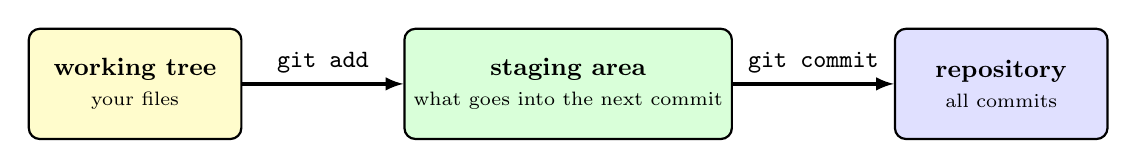
\begin{tikzpicture}[area/.style={draw, thick, rounded corners, minimum width=2.7cm, minimum height=1.4cm, align=center, font=\small}]
    \node[area, fill=yellow!20] (w) at (0,0)    {\textbf{working tree}\\ \scriptsize your files};
    \node[area, fill=green!15]  (i) at (5.5,0)  {\textbf{staging area}\\ \scriptsize what goes into the next commit};
    \node[area, fill=blue!12]   (r) at (11.0,0) {\textbf{repository}\\ \scriptsize all commits};
    \draw[-latex, very thick] (w) -- node[above, font=\ttfamily\small] {git add} (i);
    \draw[-latex, very thick] (i) -- node[above, font=\ttfamily\small] {git commit} (r);
  \end{tikzpicture}
  \end{center}
  \begin{itemize}
    \item A \textbf{commit} is a saved version of your project with a message: ``Add Hello program''.
    \item \texttt{git add} chooses \textbf{which changes} go into the next commit.
    \item \texttt{git status} always tells you where you are. \hRemark{When in doubt: \texttt{git status}.}
  \end{itemize}
\end{frame}
% ~~~~~~~~~~~~~~~~~~~~~~~~~~~~~~~~~~~~~~ A frm

% ~~~~~~~~~~~~~~~~~~~~~~~~~~~~~~~~~~~~~~ V
\hSection[First repo]{Your First Repository, Step by Step}
% ~~~~~~~~~~~~~~~~~~~~~~~~~~~~~~~~~~~~~~ A




% ~~~~~~~~~~~~~~~~~~~~~~~~~~~~~~~~~~~~~~ V frm
\begin{frame}[t,fragile] \frametitle{Step 1: \texttt{git init} makes a repository}
  \lstterminal[basicstyle=\ttfamily\scriptsize]{codeoutput/Step1.txt}

  \vspace{0.1em}
  \small
  \texttt{init} creates the hidden folder \texttt{.git}: that \emph{is} the repository. Never edit it by hand; deleting it deletes the history.
\end{frame}
% ~~~~~~~~~~~~~~~~~~~~~~~~~~~~~~~~~~~~~~ A frm




% ~~~~~~~~~~~~~~~~~~~~~~~~~~~~~~~~~~~~~~ V frm
\begin{frame}[t,fragile] \frametitle{Step 2: a file, then \texttt{git add}}
  \begin{columns}[T]
    \begin{column}{0.56\textwidth}
      \lstterminal[basicstyle=\ttfamily\tiny]{codeoutput/Step2.txt}
    \end{column}
    \begin{column}{0.4\textwidth}
      \begin{itemize}\small
        \item A new file is \textbf{untracked}: Git sees it but does not save it.
        \item \texttt{git add Hello.java}: put it into the staging area, ``to be committed''.
        \item Nothing is saved in the history yet.
      \end{itemize}
    \end{column}
  \end{columns}
\end{frame}
% ~~~~~~~~~~~~~~~~~~~~~~~~~~~~~~~~~~~~~~ A frm




% ~~~~~~~~~~~~~~~~~~~~~~~~~~~~~~~~~~~~~~ V frm
\begin{frame}[t,fragile] \frametitle{Step 3: \texttt{git commit} saves a version}
  \lstterminal[basicstyle=\ttfamily\scriptsize]{codeoutput/Step3.txt}

  \vspace{0.1em}
  \small
  \texttt{-m} gives the message. The commit gets a unique name (hash) such as \texttt{adbfbcd}; \texttt{git log} lists the commits, newest first.
\end{frame}
% ~~~~~~~~~~~~~~~~~~~~~~~~~~~~~~~~~~~~~~ A frm




% ~~~~~~~~~~~~~~~~~~~~~~~~~~~~~~~~~~~~~~ V frm
\begin{frame}[t,fragile] \frametitle{Step 4: change, look at the difference, commit again}
  \lstterminal[basicstyle=\ttfamily\tiny]{codeoutput/Step4.txt}

  \vspace{0.1em}
  \small
  \texttt{git diff}: \texttt{-} the old line, \texttt{+} the new line. \texttt{commit -a} adds all \emph{modified} tracked files (not new ones) and commits.
\end{frame}
% ~~~~~~~~~~~~~~~~~~~~~~~~~~~~~~~~~~~~~~ A frm

% ~~~~~~~~~~~~~~~~~~~~~~~~~~~~~~~~~~~~~~ V
\hSection[Java]{A Java Project in Git}
% ~~~~~~~~~~~~~~~~~~~~~~~~~~~~~~~~~~~~~~ A




% ~~~~~~~~~~~~~~~~~~~~~~~~~~~~~~~~~~~~~~ V frm
\begin{frame}[t,fragile] \frametitle{Do not commit \texttt{.class} files}
  \lstterminal[basicstyle=\ttfamily\scriptsize]{codeoutput/JavaIgnore.txt}

  \vspace{0.1em}
  \small
  \texttt{.class} files are made by \texttt{javac}: anyone can rebuild them. A one-line \texttt{.gitignore} hides them; commit the \texttt{.gitignore} itself.
\end{frame}
% ~~~~~~~~~~~~~~~~~~~~~~~~~~~~~~~~~~~~~~ A frm




% ~~~~~~~~~~~~~~~~~~~~~~~~~~~~~~~~~~~~~~ V frm
\begin{frame}[t,fragile] \frametitle{Two quick fixes: \texttt{restore} and \texttt{-{}-amend}}
  \lstterminal[basicstyle=\ttfamily\scriptsize]{codeoutput/Oops.txt}

  \vspace{0.1em}
  \small
  \texttt{git restore FILE} throws away your edits since the last commit (careful: they are gone). \texttt{-{}-amend} fixes the last commit's message.
\end{frame}
% ~~~~~~~~~~~~~~~~~~~~~~~~~~~~~~~~~~~~~~ A frm

% ~~~~~~~~~~~~~~~~~~~~~~~~~~~~~~~~~~~~~~ V
\hSection[Errors]{Common Errors}
% ~~~~~~~~~~~~~~~~~~~~~~~~~~~~~~~~~~~~~~ A




% ~~~~~~~~~~~~~~~~~~~~~~~~~~~~~~~~~~~~~~ V frm
\begin{frame}[t,fragile] \frametitle{``not a git repository''}
  \lstterminal[basicstyle=\ttfamily\scriptsize]{codeoutput/Err1.txt}

  \vspace{0.1em}
  \small
  You are in the wrong folder, or forgot \texttt{git init}. Check with \texttt{pwd} (where am I?) and \texttt{ls -a} (is there a \texttt{.git}?).
\end{frame}
% ~~~~~~~~~~~~~~~~~~~~~~~~~~~~~~~~~~~~~~ A frm




% ~~~~~~~~~~~~~~~~~~~~~~~~~~~~~~~~~~~~~~ V frm
\begin{frame}[t,fragile] \frametitle{``nothing added to commit''}
  \lstterminal[basicstyle=\ttfamily\scriptsize]{codeoutput/Err2.txt}

  \vspace{0.1em}
  \small
  \texttt{commit} only saves what is \textbf{staged}. Read Git's hint: \texttt{git add notes.txt} first.
\end{frame}
% ~~~~~~~~~~~~~~~~~~~~~~~~~~~~~~~~~~~~~~ A frm




% ~~~~~~~~~~~~~~~~~~~~~~~~~~~~~~~~~~~~~~ V frm
\begin{frame}[t,fragile] \frametitle{``Please tell me who you are''}
  \lstterminal[basicstyle=\ttfamily\tiny]{codeoutput/Err3.txt}

  \vspace{0.1em}
  \small
  Git refuses to commit without a name and e-mail: run the two \texttt{git config -{}-global} lines from the beginning of this deck.
\end{frame}
% ~~~~~~~~~~~~~~~~~~~~~~~~~~~~~~~~~~~~~~ A frm




% ~~~~~~~~~~~~~~~~~~~~~~~~~~~~~~~~~~~~~~ V frm
\begin{frame}[t,fragile] \frametitle{``pathspec did not match any files''}
  \lstterminal[basicstyle=\ttfamily\scriptsize]{codeoutput/Err4.txt}

  \vspace{0.1em}
  \small
  A typo in the file name. On Linux \texttt{Readme.md} $\neq$ \texttt{README.md}; on \win{} and \mac{} file names usually ignore case, so the first command might work there. Use \keys{Tab} to complete names.
\end{frame}
% ~~~~~~~~~~~~~~~~~~~~~~~~~~~~~~~~~~~~~~ A frm




% ~~~~~~~~~~~~~~~~~~~~~~~~~~~~~~~~~~~~~~ V frm
\begin{frame}[t,fragile] \frametitle{``src refspec main does not match any''}
  \lstterminal[basicstyle=\ttfamily\scriptsize]{codeoutput/Err5.txt}

  \vspace{0.1em}
  \small
  You tried to push a branch that has no commits yet. Commit something first, then push.
\end{frame}
% ~~~~~~~~~~~~~~~~~~~~~~~~~~~~~~~~~~~~~~ A frm

% ~~~~~~~~~~~~~~~~~~~~~~~~~~~~~~~~~~~~~~ V
\hSection[Summary]{Summary}
% ~~~~~~~~~~~~~~~~~~~~~~~~~~~~~~~~~~~~~~ A




% ~~~~~~~~~~~~~~~~~~~~~~~~~~~~~~~~~~~~~~ V frm
\begin{frame}[t,fragile] \frametitle{Cheat sheet}
  \begin{columns}[T]
    \begin{column}{0.56\textwidth}
      \begin{center}\footnotesize
      \begin{tabular}{ll}
        \toprule
        \textbf{I want to \dots}      & \textbf{command} \\
        \midrule
        start a repository           & \texttt{git init} \\
        see what changed             & \texttt{git status}, \texttt{git diff} \\
        choose files to save         & \texttt{git add FILE} \\
        save a version               & \texttt{git commit -m "message"} \\
        see the history              & \texttt{git log -{}-oneline} \\
        throw away my edits          & \texttt{git restore FILE} \\
        fix the last message         & \texttt{git commit -{}-amend -m "\dots"} \\
        \bottomrule
      \end{tabular}
      \end{center}
    \end{column}
    \begin{column}{0.4\textwidth}
      \begin{block}{Do}
        \small commit often, with clear messages; \texttt{git status} before and after every step; ignore build files
      \end{block}
      \begin{block}{Don't}
        \small commit \texttt{.class} files or passwords; edit \texttt{.git}; put a repository inside another one
      \end{block}
    \end{column}
  \end{columns}
\end{frame}
% ~~~~~~~~~~~~~~~~~~~~~~~~~~~~~~~~~~~~~~ A frm




% ~~~~~~~~~~~~~~~~~~~~~~~~~~~~~~~~~~~~~~ V frm
\begin{frame}[t,fragile] \frametitle{Exercises}
  \begin{enumerate}\small
    \item Install Git, set your name and e-mail, and check with \texttt{git config -{}-global -{}-list}.
    \item Create a repository for your next homework. Commit after each exercise you finish.
    \item Add a \texttt{.gitignore} with \texttt{*.class}. Compile, then check that \texttt{git status} stays clean.
    \item Change a line, look at \texttt{git diff}, then \texttt{git restore} it. Is the change really gone?
    \item Make each error of section 5 happen on your own computer and read the message carefully.
  \end{enumerate}
\end{frame}
% ~~~~~~~~~~~~~~~~~~~~~~~~~~~~~~~~~~~~~~ A frm




% ~~~~~~~~~~~~~~~~~~~~~~~~~~~~~~~~~~~~~~ V frm
\begin{frame}[t,fragile]
	\begin{center}
		\vspace{4cm}
		\hRemark{\Huge Questions?}
	\end{center}
\end{frame}
% ~~~~~~~~~~~~~~~~~~~~~~~~~~~~~~~~~~~~~~ A frm



\end{document}
